% Chapter 4

\chapter{Code Refactoring}

\lhead{Chapter 4. \emph{Code Refactoring}} % This is for the header on each page - perhaps a shortened title
\label{chp:refwork}
%----------------------------------------------------------------------------------------

\def\:{\hskip0pt} %Definisce un modo veloce per permettere a latex di sillabare correttamente anche parole come 4-connectivity. Il corretto utilizzo è il seguente: 4\:-\:connectivity.
\section{Introduction}
Cipriano et al. spent some effort to develop the dataset and a to design a
network which was capable to perform the segmentation of the Inferior Alveolar
Canal.
Together with the novel dataset, they proposed a modified version of
U-Net 3D as a back-bone for both the label propagation and the IAC segmentation.
Both of these network and method were introduced in the previous
chapters and will be explained more in details in the following sections.
As the code was written near the deadline for the submission of the paper,
the authors did not have focused on producing a codebase which was optimized for
reusability, extensibility and efficiency.
For this reason, my work start by refactoring the codebase to add these features
which improved all my successive experiments.

\section{Reference Work}
The pipeline proposed can be divided in two main steps: the deep label
propagation and the IAC segmentation.

\subsection{Positional PadUNet3D}
A slightly modified version of 3D U-Net has been proposed as a backbone for both
steps. Differently from the original 3D U-Net architecture, every
three-dimensional convolution in our CNN applies a 2 pixels padding along each
dimension. Although this alteration does not cause any variation in terms of
performance, it ensures that the output of each convolution has the same size of
its input along axis \emph{x}, \emph{y}, and \emph{z}.

Resolution changes are therefore due uniquely to the
three max pooling layers, each halving the size of the
volumes. When using the aforementioned input size, the
encoder output is composed of $512$ feature maps of size
$10 \times 10 \times 10$. Inside the decoder, on the other hand, resolution changes are caused by transposed convolutions, with
dimensions $2 \times 2 \times 2$ for both the kernel and stride to double the size of the feature maps. This adjustment ensures
resolution symmetry between features in the decoder and
corresponding maps in the encoder, thus allowing them to
be simply concatenated with skip connections. Moreover,
the output of the model naturally has the same dimensions
of the input. The final output is a single channel volume, to
which we apply a Sigmoid activation function and a threshold at $0.5$ to obtain the final binary prediction mask.

The segmentation architecture is further enriched with a
positional embedding. Since our sub-volumes are extracted
from the original scan following a fixed grid, we exploit
positional information derived from the location of the topleft and bottom-right corners of the sub-volume. Specifically, these global coordinates are fed to a linear layer which
yields a single feature map of dimensions $10 \times 10 \times 10$. This
positional embedding gets concatenated to the output of the
encoder, and then fed to the decoder. Exploiting positional
information ensures two extremely important benefits:
\begin{itemize}
  \item{During training, the CNN is fed with implicit information about areas
  close to the edges of the scan, where the IAN is very unlikely to be present.
  This piece of knowledge greatly reduces the number of false positives during
  inference. As a matter of fact, no postprocessing method is required to refine
  the output of the proposed CNN}
  \item{Information about cut positions helps the network to better shape the
  output: sub-volumes located close to the mental foramen generally present a
  much thinner canal than those located in the mandibular foramen. This
  technique could indeed be employed for several classes of medical data, as
  anatomical structures can substantially vary according to their location.}
\end{itemize}

\subsection{Deep Label Propagation}
The presence of a new 3D voxel-level annotated dataset paves the way to a new
frontier for label propagation: we can indeed employ 3D annotations to supervise
a deep label propagation neural network, trained to expand sparse labels into
dense ones, and produce high quality synthetic ground truths for the
segmentation task. We christen this new label propagation approach Deep Label
Expansion, or Deep Expansion in short. The deep expansion model is based on the
proposed segmentation network, Positional PadUNet. The main difference regards
the input layer, that is changed in order to accept a concatenation of both the
raw volume data and the sparse annotations, rendered as a binary channel. Thus,
the network input has a shape of $2 \times 80 \times 80 \times 80$. Same as
Positional PadUNet, a positional embedding is concatenated to the encoder
output. By means of this model, we generate a synthetic dataset which will be
employed to pre-train our final segmentation CNN. Once again, the positional
embedding supplies important information about the location of the cut, which is
closely related to the diameter of the expanded labeled canal.

\section{Refactoring}
The code was divided in two main repositories, one for the label propagation and
one for the IAC segmentation. For this reason, a lot of code was duplicated and
a single repository was created to host all the codebase. Moreover, the code has been
rewritter from scratch, and only some parts of the original codebase have been
copied.
% restructured to allow the user to easily change the parameters of the network

\subsection{Data Loading}
The first issue tackled was the lack of use of TorchIO classes as abstraction
for the new proposed dataset. The original codebase was using a custom class which
was responsible to load the data, compute some statistics and to read part of
the config file to select which transformation apply to perform the data
augmentation. Moreover, custom transformation functions were defined here in the
same file.

One of the main advantages of using TorchIO is that it provides three main
datastructures which are used to represent the data: \emph{Image},
\emph{Subject} and \emph{SubjectsDataset}.

The Image class, representing one medical image, stores a 4D tensor, whose
voxels encode, e.g., signal intensity or segmentation labels, and the
corresponding affine transform, typically a rigid (Euclidean) transform, to
convert voxel indices to world coordinates in mm. Arbitrary fields such as
acquisition parameters may also be stored. Subclasses are used to indicate
specific types of images, such as \emph{ScalarImage} and \emph{LabelMap}, which
are used to store, e.g., CBCT scans and segmentations, respectively.

The Subject is a data structure used to store images associated with a subject
and any other metadata necessary for processing. It is essential to link a
ScalarImage to its relative LabelMaps.

The SubjectsDataset is a subclass of torch.utils.data.Dataset which is used to
store a collection of Subject. It can be used with PyTorch DataLoader for
efficient loading and augmentation. The figure \ref{fig:subjectsdataset}
depicts the relation between these classes.
\begin{figure}[h]
  \centering
  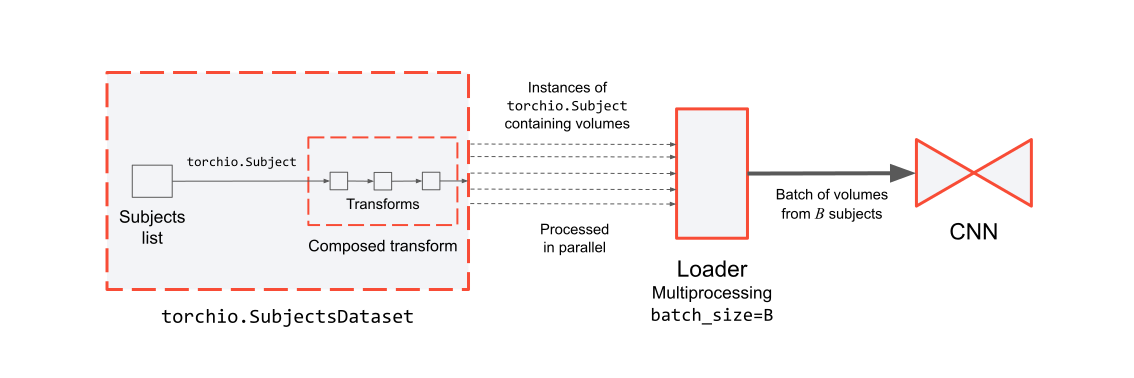
\includegraphics[width=0.8\linewidth]{Images/subjectsdataset.png}
  \caption{SubjectsDataset class}
  \label{fig:subjectsdataset}
\end{figure}
With these data structures, a Maxillo class, which inherith from
SubjectsDataset, has been created to load the data. This class take as input the
path of the dataset, which split to load (train, validation, test, synthetic)
and optionally a list of Transformations that must be used as data
augmentations. This class is completely indipendent from the rest of the code,
thus can be used in any other project which requires to load the maxillo
dataset.

\subsection{Data Augmentation}
Transformation functions which were previously defined in the same file of the
data loader have been moved in a new file. Some of them were already implemented
inside TorchIO and thus have been removed. The remaining ones have been adapted
to inherith from the abstract \texttt{class torchio.transforms.Transform}, in
order to be easly used inside TorchIO, such with the \emph{Composability} method
which allow to create a directed acyclic graph of transformations that must be
applied to the data.

\subsection{Config and command line arguments}
In the original codebase, the parameters of the program were passed both as
arguments from the command line and in the config file. This could generate some
confusion and make harder to reproduce an experiments as the config file alone
wasn't enough. For this reason, the config file is now the only source of
parameters, while the only arguments that the software accepts are the path of the
config file and a boolean value to enable/disable Tensorflow.
An example of config file is shown below:

\begin{lstlisting}[language=YAML,breaklines=true,caption=Example of config file., label=union]
title: 'canal_generator_train'
project_dir: '/homes/llumetti/results'
seed: 47
tensorboard_dir: '/homes/llumetti/tensorboard'

experiment:
  name: 'Generation'

data_loader:
  dataset: '/nas/softechict-nas-1/llumetti/maxillo'
  augmentations: 'configs/augmentations.yaml'
  background_suppression: 0
  batch_size: 2
  labels:
    BACKGROUND: 0
    INSIDE: 1
  mean: 0.08435
  num_workers: 8
  patch_shape:
  - 120
  - 120
  - 120
  resize_shape:
  - 168
  - 280
  - 360
  sampler_type: grid
  grid_overlap: 0
  std: 0.17885
  volumes_max: 2100
  volumes_min: 0
  weights:
  - 0.000703
  - 0.999

model:
  name: 'PosPadUNet3D'

loss:
  name: 'Jaccard'

lr_scheduler:
  name: 'Plateau'

optimizer:
  learning_rate: 0.1
  name: 'SGD'

trainer:
  reload: False
  checkpoint: null
  do_train: False
  do_test: False
  do_inference: True
  epochs: 100
\end{lstlisting}

\subsection{Interfaces}
Something about interfaces used for Models, Losses, Optimizers, Schedulers and
Experiments...

\subsection{Deploying and Running}
The code was managed using Git and the repository is hosted on GitHub the
repository is public and can be found at \url{https://github.com/AImageLab-zip/alveolar\_canal}.
By using Git, it was possible to easly deploy the code on the AImagelab Server by
means of a simple script which keeps the code up to date with the main branch.
Other branches were used to develop new features and to test them before merging
everything in the main branch. The Gitflow workflow was used to manage the
branches. The training was scheduled using the SLURM scheduler, which is
installed on the server. Some scripts were written to automatize the training
process, which often required to run sequentially multiple experiments with
different configurations file and to recover training from a given checkpoint
when the training was long and the scheduler kill the process for exceeding the
time limit.
